% 04_product_space.tex
%! TeX root = ../main.tex

\chapter{Esperimenti congiunti}

\section{Prodotto di spazi di probabilità}

Supponiamo di svolgere due esperimenti aleatori diversi, rappresentati dai due spazi di probabilità $\left( \Omega_1, \mathcal{F}_1, \mathbb{P}_1 \right)$ e $\left( \Omega_2, \mathcal{F}_2, \mathbb{P}_2 \right)$. 
Per fare previsioni, è del tutto lecito cercare di modellizzarli complessivamente come un solo esperimento, detto \textit{congiunto}. Per produrre uno spazio di probabilità, prima costruiremo uno spazio strutturato, e poi introdurremo una misura. 

\subsection{Prodotto di spazi misurabili}
Partiamo dall'insieme degli esiti $\Omega$: che nel primo esperimento si verifichi un certo esito e nel secondo un altro è del tutto equivalente al verificarsi di un esito "bidimensionale" che contenga come prima coordinata l'esito del primo esperimento e come seconda coordinata l'esito del secondo. 
In altri termini, $\Omega$ è in bigezione con $\Omega_1 \times \Omega_2$: quindi, scegliamo proprio il prodotto per rappresentare l'esperimento congiunto:
\[
	\Omega = \Omega_1 \times \Omega_2.	
\]

A questo punto, stabiliamo una struttura $\sigma$-additiva che dia concretezza ai predicati sugli esiti: imponiamo su $\Omega_1 \times \Omega_2$ una $\sigma$-algebra $\mathcal{A}$.
Ovviamente, vogliamo poterci ridurre a studiare i due esperimenti singolarmente, e quindi è necessario che per $E \in \mathcal{F}_1$ si abbia che $E \times \Omega_2 \in \mathcal{A}$. 
Non solo: stiamo considerando l'esperimento congiunto proprio per studiare le relazioni tra i due esperimenti, quindi un altro requisito è che se $E_1 \in \mathcal{F}_1$ e $E_2 \in \mathcal{F}_2$ allora $E_1 \times E_2 \in \mathcal{A}$. 
Poichè la collezione $\left\{ E_1 \times E_2 : E_i \in \mathcal{F}_i \text{ for } i=1,2 \right\}$, detta "collezione dei rettangoli", non è una $\sigma$-algebra, considereremo come struttura dell'esperimento congiunto
\[
	\mathcal{F}_1 \otimes \mathcal{F}_2 = \sigma \left( \left\{ E_1 \times E_2 : E_i \in \mathcal{F}_i \text{ for } i=1,2 \right\} \right),
\]
e cioè la più piccola\footnote{Per quelli che non hanno ancora bevuto il caffè mattutino, questo è desiderabile perchè più spazzatura aggiungiamo, più si restringe la classe di probabilità che potremo definirci sopra.
Un esempio: la probabilità uniforme può essere definita su $\mathcal{B}([0,1])$, ma non su $\mathcal{P}([0,1])$.} $\sigma$-algebra che contiene gli esiti di interesse. Diamo un'intuizione considerando il caso $\left( \Omega_i, \mathcal{F}_i \right) = \left( \mathbb{R}, \mathcal{B}(\mathbb{R}) \right)$ illustrato in Figura \ref{fig}. 

\begin{figure}[H]

% figures	
	\begin{subfigure}{.3\textwidth}

		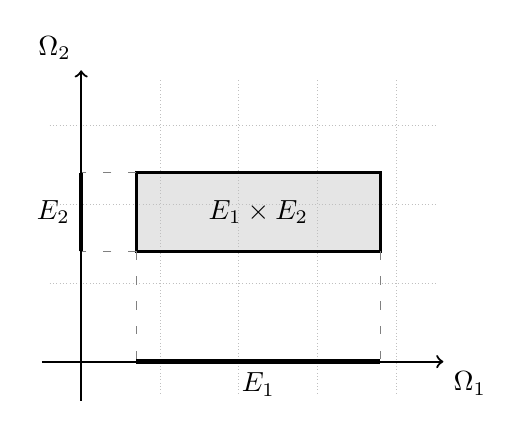
\begin{tikzpicture}
			% shape colour
			\fill[gray!20!white] (0.7,1.4) -- (3.8,1.4) -- (3.8,2.4) -- (0.7,2.4) -- cycle;
	
			% grid
			\draw[step=1, gray!50!white, densely dotted, very thin] (-.4,-.4) grid (4.5,3.6);
	
			%shapes
			\draw[very thick] (0.7,1.4) rectangle (3.8,2.4) node [midway] {$E_1 \times E_2$};
			\draw[ultra thick] (0,1.4) -- node [anchor=east]{$E_2$} (0,2.4);
			\draw[ultra thick] (0.7,0) -- node [anchor=north]{$E_1$} (3.8,0);
			\draw[loosely dashed, gray] (0.7,1.4) -- (0,1.4);
			\draw[loosely dashed, gray] (0.7,1.4) -- (0.7,0);
			\draw[loosely dashed, gray] (3.8,1.4) -- (3.8,0);
			\draw[loosely dashed, gray] (0.7,2.4) -- (0,2.4);
	
			% axis
			\draw[thick, ->] (0,-.5) -- (0,3.6+0.1) node [anchor=south east]{$\Omega_2$};
			\draw[thick, ->] (-.5,0) -- (4.5+.1,0) node [anchor=north west]{$\Omega_1$};
		\end{tikzpicture}
		\caption{Un insieme della collezione dei rettangoli.}			\label{figa}	
	\end{subfigure}
	\hfill
	\begin{subfigure}{.3\textwidth}

		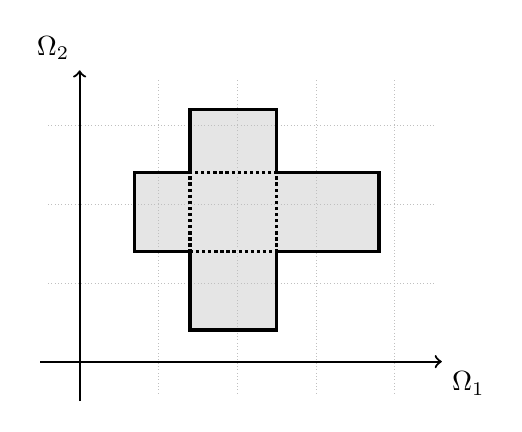
\begin{tikzpicture}
			% shape colour
			\fill[gray!20!white] (0.7,1.4) -- (3.8,1.4) -- (3.8,2.4) -- (0.7,2.4) -- cycle;
			\fill[gray!20!white] (1.4,.4) -- (2.5,.4) -- (2.5,3.2) -- (1.4,3.2) -- cycle;

			% grid
			\draw[step=1, gray!50!white, densely dotted, very thin] (-.4,-.4) grid (4.5,3.6);

			%shapes
			\draw[very thick] (0.7,1.4) -- (1.4,1.4) -- (1.4,.4) -- (2.5,.4) -- (2.5,1.4) -- (3.8,1.4) -- (3.8,2.4) -- (2.5,2.4) -- (2.5,3.2) -- (1.4,3.2) -- (1.4,2.4) -- (.7,2.4) -- cycle;
			\draw[very thick, densely dotted] (1.4,1.4) -- (2.5,1.4) -- (2.5,2.4) -- (1.4,2.4) -- cycle;
	
			% axis
			\draw[thick, ->] (0,-.5) -- (0,3.6+0.1) node [anchor=south east]{$\Omega_2$};
			\draw[thick, ->] (-.5,0) -- (4.5+.1,0) node [anchor=north west]{$\Omega_1$};
		\end{tikzpicture}
		\caption{L'unione di due rettangoli che non sia un rettangolo.}				\label{figb}
	\end{subfigure}
	\hfill
	\begin{subfigure}{.3\textwidth}

		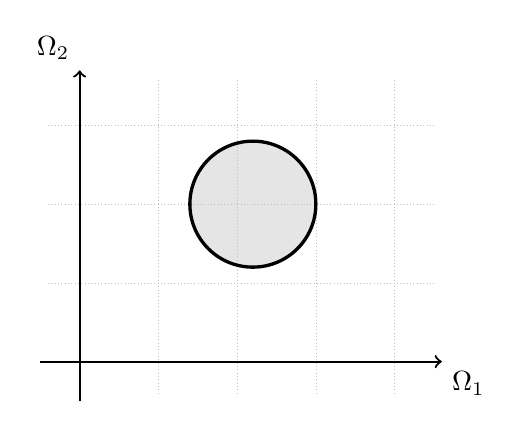
\begin{tikzpicture}
			% shape colour
			\fill[gray!20!white] (2.2,2) circle [radius = 0.8];
	
			% grid
			\draw[step=1, gray!50!white, densely dotted, very thin] (-.4,-.4) grid (4.5,3.6);
	
			%shapes
			\draw[very thick] (2.2,2) circle [radius = 0.8];
	
			% axis
			\draw[thick, ->] (0,-.5) -- (0,3.6+0.1) node [anchor=south east]{$\Omega_2$};
			\draw[thick, ->] (-.5,0) -- (4.5+.1,0) node [anchor=north west]{$\Omega_1$};
		\end{tikzpicture}
		\caption{Un evento che non sia un rettangolo.}			\label{figc}	
	\end{subfigure}
	\caption{Esempi di eventi in $\mathcal{F}_1 \otimes \mathcal{F}_2$, per $\Omega_i=\mathbb{R}$ e $\mathcal{F}_i = \mathcal{B}(\mathbb{R})$.}	\label{fig}
\end{figure}	
Il generico insieme della collezione dei rettangoli $E_1 \times E_2$ può essere rappresentato come in Figura \ref{figa}, in accordo con l'idea di rettangolo\footnote{Achtung: anche l'insieme $\mathbb{Q}^2$, per esempio, appartiene a questa collezione, ma la sua rappresentazione geometricamente non è un rettangolo.}. 
Pertanto, i due insiemi in Figura \ref{figb} sono entrambi appartenenti alla collezione, ma la loro unione evidentemente no: questo esemplifica come la collezione dei rettangoli può fallire ad essere una $\sigma$-algebra. 
Ma $\mathcal{F}_1 \otimes \mathcal{F}_2$ contiene anche insiemi più complessi: la Figura \ref{figc} mostra un evento di questa $\sigma$-algebra.
\par Infine, alcune considerazioni. In primo luogo, quanto visto può essere facilmente esteso a più di due spazi procedendo iterativamente.
\par Inoltre, un risultato notevole è che definendo la $\sigma$-algebra di Borel di $\mathbb{R}^n$ come quella generata dalla topologia, e cioè $\mathcal{B}\left(\mathbb{R}^n\right) \defeq \sigma(\mathcal{T}_\mathbb{R^n})$, si ottiene che $\otimes^n \mathcal{B}(\mathbb{R}) = \mathcal{B}\left(\mathbb{R^n}\right)$. Questo conferma la buona definizione dello spazio prodotto e, per le prossime sezioni, motiva il fatto che comunemente i vettori di variabili aleatorie siano definiti su $\left(\mathbb{R}^n,\mathcal{B}(\mathbb{R}^n)\right)$.

\subsection{Prodotto di misure di probabilità}
Finora, le scelte sono state fatte in maniera obbligata: se avessimo considerato oggetti diversi da $\times \Omega_i$ e $\otimes \mathcal{F}_i$ la descrizione dello spazio misurabile sarebbe stata logicamente equivalente\footnote{E cioè tutto sarebbe stato identico ai fini modellistici, "modulo" una bigezione.}, o avrebbe perso di flessibilità o di informazione.

Per la misura di probabilità $\mathbb{P}$ su questo spazio, non avremo lo stesso lusso: infatti, l'unico requisito che possiamo imporre è quello di consistenza con gli spazi di partenza. 
Formalmente, che per $E_1 \in \mathcal{F}_1$ si abbia
\[
	\mathbb{P}_1(E_1) = \mathbb{P} (E_1 \times \Omega_2),
\]
e analogamente per $E_2 \in \mathcal{F}_2$. 
Si può dimostrare che esistono più misure di probabilità con questa caratteristica: possiamo garantire l'unicità solo con ulteriori vincoli modellistici e, in particolare, è sufficiente che gli esperimenti marginali siano indipendenti\footnote{Ricordiamo che $A \perp B$ se e solo se $\mathbb{P}(A \cap B) = \mathbb{P}(A) \mathbb{P}(B)$}, e cioè valga la fattorizzazione
\[
	\mathbb{P} (E_1 \times \Omega_2 \cap \Omega_1 \times E_2) = \mathbb{P} (E_1 \times \Omega_2) \mathbb{P} (\Omega_1 \times E_2).
\]
Poichè $E_1 \times \Omega_2 \cap \Omega_1 \times E_2 = E_1 \times E_2$, possiamo imporre il requisito come segue.
\begin{my_theorem}
	Siano $\left( \Omega_1, \mathcal{F}_1, \mathbb{P}_1 \right)$ e $\left( \Omega_2, \mathcal{F}_2, \mathbb{P}_2 \right)$ due spazi di probabilità. 
	Allora esiste ed è unica la probabilità $\mathbb{P}$ su $\left(\Omega_1 \times \Omega_2, \mathcal{F}_1 \otimes \mathcal{F}_2\right)$ tale che
	\[
		\mathbb{P} (E_1 \times E_2) = \mathbb{P}_1 (E_1) \mathbb{P}_2 (E_2)
	\]
	per $E_1 \in \mathcal{F}_1$ e $E_2 \in \mathcal{F}_2$. 
	Chiamiamo $\mathbb{P}$ la "probabilità prodotto" e la indichiamo con $\mathbb{P}_1 \otimes \,\mathbb{P}_2$.
\end{my_theorem}

Una proprietà desiderabile di $\mathbb{P}_1 \otimes \,\mathbb{P}_2$ è la computabilità.
Sia $C \in \mathcal{F}_1 \otimes \mathcal{F}_2$, e siano le "sezioni" di $C$ definite come segue:
\[
	C_1 (\omega_2) = \{ \omega_1 \in \Omega_1 : (\omega_1,\omega_2) \in C \} \qquad
	C_2 (\omega_1) = \{ \omega_2 \in \Omega_2 : (\omega_1,\omega_2) \in C \}	
\]
Allora, le funzioni "probabilità della sezione"
\begin{gather*}
	\omega_1 \in \Omega_1 \longmapsto  \mathbb{P}_2 ( C_2 (\omega_1)) \in \mathbb{R} \\
	\omega_2 \in \Omega_2 \longmapsto  \mathbb{P}_1 ( C_1 (\omega_2)) \in \mathbb{R}
\end{gather*}
sono misurabili e limitate, e quindi integrabili.
Questo conferma la buona posizione della regola
\begin{align*}
	(\mathbb{P}_1 \! \otimes \mathbb{P}_2) (C) &= \! \int\limits_{\Omega_1\times\Omega_2} \mathbb{1}_C(\boldsymbol{\omega}) \, \mathbb{P}_1 \! \otimes \mathbb{P}_2(\mathrm{d}\boldsymbol{\omega}) = \\
	&= \int\limits_{\Omega_1} \mathbb{P}_2(C_2(\omega_1)) \, \mathbb{P}_1 (\mathrm{d}\omega_1).
\end{align*}
\begin{proof}
	Proveremo un solo caso. Sia $C = E_1 \times E_2$ con $E_i \in \mathcal{F}_i$. Si dimostra che $\pi_2 : (\omega_1,\omega_2) \in \Omega_1 \times \Omega_2 \to \omega_2 \in \Omega_2$ è misurabile ed integrabile. Allora,
	\begin{align*}
		\mathbb{P}_1 \otimes \, \mathbb{P}_2 (E_1 \times E_2) &
			= \mathbb{P}_1(E_1)\mathbb{P}_2(E_2) = \\
			& = \mathbb{P}_1(E_1) \mathbb{E}_{\mathbb{P}_2}[\mathbb{1}_{E_2}]
			= \mathbb{P}_1(E_1) \mathbb{E}_{\otimes\mathbb{P}}[\mathbb{1}_{E_2} \circ \pi_2]= \\
			& = \int_{\Omega_2} \mathbb{P}_1(E_1) \mathbb{1}_{E_2}(\omega_2) \mathbb{P}_2(\mathrm{d}\omega_2).
	\end{align*}
	Poichè se $\omega_2 \in E_2$ allora $C_1(\omega_2)=\{ \omega_1 \in \Omega_1 : (\omega_1,\omega_2) \in C = E_1 \times E_2 \}=E_1$, si ha che $t_2(\omega_2) = \mathbb{P}(E_1)$. Similmente, se $\omega_2 \notin E_2$, allora $C_1(\omega_2)=\emptyset$ e $t_2(\omega_2) = 0$. Quindi, $t_2 = \mathbb{P}_1(E_1) \mathbb{1}_{E_2}$, da cui segue la tesi. Per linearità, segue il caso di $C=\bigcup^n E_{1,i} \times E_{2,i}$ con $E_{2,i}$ disgiunti (se non lo sono, si può recastare il set in una sommatoria dove lo sono). Infine, per $C$ generico, è sufficiente trovare un'approssimante $C^{(n)}=\bigcup^n E_{1,i}^{(n)} \times E_{2,i}^{(n)}$ dal basso (?? esplicitarla ??), e osservare che per continuità monotona di $\otimes \mathbb{P}$ e MCT applicato alla sequenza $t_2^{(n)} \big\uparrow t_2$ segue la tesi in generale.
\end{proof}
Ovviamente, anche in questo caso tutto si può estendere a più di due spazi iterativamente.

\section{Vettori aleatori e prodotto di spazi}

Rimangono da introdurre le variabili aleatorie su o da spazi prodotto. Per farlo, in primo luogo stabiliamo dei criteri di misurabilità. Poi, discuteremo un criterio di indipendenza e infine troveremo un regola computazionale per il valore atteso.

\subsection{Misurabilità}

La situazione più semplice, quella in cui date delle variabili aleatorie definite sullo stesso spazio ci chiediamo come si comporta il loro vettore, è stata già incontrata nel caso di vettori aleatori reali: il vettore era misurabile se e solo lo erano le componenti. 
A conferma\footnote{Che il criterio valesse per i vettori reali lo rende \textit{desiderabile} in generale} della buona definizione dello spazio prodotto, questa proprietà continua a valere.
\begin{my_lemma}[Misurabilità delle componenti]
	Per $X: \Omega \to E$, $Y: \Omega \to E$, si ha che $X:(\Omega,\mathcal{A}) \to (E,\mathcal{E})$ e $Y:(\Omega,\mathcal{A}) \to (E,\mathcal{F})$ sono misurabili se e solo se lo è $(X,Y):(\Omega,\mathcal{A}) \to (E \times F,\mathcal{E} \otimes \mathcal{F})$.
\end{my_lemma}

La seconda casistica, quella in cui il dominio è uno spazio prodotto, è più delicata e l'implicazione vale solo in un verso. 
Per fissare le idee, consideriamo solo un caso.
\begin{my_lemma}[Misurabilità delle restrizioni]
	Sia $X : (\Omega_1 \times \Omega_2, \mathcal{F}_1 \otimes \mathcal{F}_2) \to (\mathbb{R}, \mathcal{B}(\mathbb{R}))$ un vettore aleatorio. Allora, la restrizione
	\[
		X(\boldsymbol{\cdot},\omega_2):\Omega_1 \to \mathbb{R}
	\]
	è misurabile per ogni $\omega_2 \in \Omega_2$ rispetto a $\mathcal{F}_1$.
\end{my_lemma}
Questa è solo una condizione necessaria e non un criterio per la misurabilità: non vale l'inverso. 
Esplicitamente, la misurabilità di $X(\cdot,\omega_2)$ e $X(\omega_1, \cdot)$ rispetto ad ogni $\omega_1 \in \Omega_1$ e $\omega_2 \in \Omega_2$ non implica quella del vettore (come ci si potrebbe aspettare\dots).

Ciò detto il risultato caratterizza gli insiemi misurabili dello spazio prodotto: se $C \in \otimes \mathcal{F}_i$ allora $X = \mathbb{1}_C$ è misurabile, la restrizione $\mathbb{1}_C(\boldsymbol{\cdot},\omega_2)$ è misurabile, e la sezione $C_1(\omega_2)$ è un evento\footnote{Questo prova quanto visto nella regola per computare $\otimes \mathbb{P}$}. 
In altri termini, tutte le "sezioni" di un insieme misurabile nello spazio prodotto sono misurabili rispetto agli spazi marginali.

\subsection{Criterio di Indipendenza}

Supponiamo di considerare gli esperimenti $(E_i, \mathcal{E}_i, \mathbb{P}_i)$ congiuntamente, ed imponiamo che siano indipendenti: per quanto visto, consideriamo cioè la misura prodotto $\otimes \mathbb{P}_i$ su $(\times E_i, \otimes \mathcal{E}_i)$.
Ora \textit{accendiamo} le variabili aleatorie: se ognuno di questi spazi fosse lo spazio immagine di un solo esperimento $(\Omega,\mathcal{F},\mathbb{P})$ attraverso $X_i : \Omega \to E_i$, allora avremmo che
\[
	X=(X_1,\dots,X_n) : \Omega \to E_1 \times \dots \times E_n.
\]

Facciamo un ragionamento modellistico: che gli spazi iniziali considerati congiuntamente fossero indipendenti significa che la conoscenza di un evento su uno non influenza le predizioni di un evento sull'altro. 
Introducendo le variabili aleatorie, lasciamo la struttura delle dipendenze inalterata, quindi sarebbe desiderabile che la conoscenza di un evento su uno spazio immagine non influenzasse le previsioni degli eventi sugli altri spazi immagine. 

In altri termini, se le definizioni fossero ben poste dovremmo avere l'indipendenza delle variabili aleatorie, e cioè (nel caso $n=2$)
\[
	P_{(X_1,X_2)} (E_1 \times E_2) = \mathbb{P} \{X_1 \in E_1, X_2 \in E_2 \} = \mathbb{P} \{X_1 \in E_1\} \mathbb{P} \{X_2 \in E_2 \} = P_{X_1} (E_1) P_{X_2} (E_2).
\]
Questo è confermato dal seguente risultato, per cui vale anche l'inverso: se le variabili aleatorie sono indipendenti, allora il loro vettore è definito sullo spazio prodotto.
% Due variabili aleatorie definite sullo stesso esperiemnto sono indipendenti se il verificarsi di un evento su una non non informa le predizioni sugli eventi dell'altra. Formalmente, se gli eventi E_1 si è verificato l'evento A dello spazio di X_1, e cioè E_1=X_1^{-1}(A) ed E_2 similmente definito sono indipendenti rispetto allo spazio di partenza. In altri termini, se le sub-sigma-alg sigma(X_1) e sigma(X_2) sono indipendenti. Per essere espliciti, stiamo imponendo che P fattorizzi rispetto agli eventi {X_1 in A} e {X_2 in B}.
\begin{my_lemma}
	\label{equival_indip}
	Le variabili aleatorie $X:\Omega \to E$ e $Y:\Omega \to F$ sono indipendenti se e solo se 
	\begin{equation}
		\label{crit}
		P_{(X,Y)} = P_X \otimes P_Y.	
	\end{equation}
\end{my_lemma}
A livello operativo, questo risultato ha due conseguenze. In primo luogo, è un criterio per stabilire se due variabili aleatorie sono indipendenti: è necessario e sufficiente che la probabilità congiunta fattorizzi nelle probabilità marginali per ogni scelta di eventi negli spazi di arrivo.

La seconda è che permette di provare il seguente lemma, che a sua volta conferma che è sufficiente informare sulla legge di ogni variabile $X_i$ e dire che sono indipendenti perchè esista un'unica variabile aleatoria nello spazio prodotto con queste caratteristiche.

\begin{my_lemma}
	Siano $X_i : \Omega \to (E_i, \mathcal{E}_i, P_i)$ variabili aleatorie. Allora, il vettore $X=(X_1,\dots,X_n):\Omega \to (\times E_i, \otimes \mathcal{E}_i, \otimes P_i)$ è tale che 
	\begin{itemize}
		\item La sua $i$-esima componente è distribuita come $X_i$: in simboli, $(X)_i \sim X_i$,
		\item Le sue componenti sono una famiglia di variabili aleatorie indipendenti.
	\end{itemize}
\end{my_lemma}

Lasciamo in appendice al capitolo la dimostrazione di \ref{equival_indip}.

\begin{proof}[?? da sistemare]
	Osserviamo che \ref{crit} vale se e solo se $P_{(X,Y)} (A \times B) = P_X(A) P_Y(B)$ per ogni $A\in\mathcal{E}$ e $B\in\mathcal{F}$. Consideriamo $P_{(X,Y)} (A \times B) = \mathbb{P}(\{X \in A\},\{Y \in B\}) = \mathbb{P}\{X \in A\} \mathbb{P} \{Y \in B\}$. Se le r.v. sono indipendenti, percorrerla da sinistra dimostra la tesi; se vale \ref{crit} è sufficiente osservare che si ottine la def di indipendendenza stocastica.
\end{proof}

\subsection{Teorema di Fubini-Tonelli}

Tornando al caso di variabili aleatorie definite sul prodotto di spazi, il calcolo del valore atteso diventa un'estensione dell'integrale multivariabile. 
Operativametne, potremmo ragionare in termini di integrale di Riemann multivariabile ma, come vedremo, ha più senso ricondursi all'integrale astratto in una sola variabile, e solo a quel punto impiegare l'integrale di Riemann.

In particolare, sotto positività o integrabilità, è possibile calcolare l'integrale sullo spazio prodotto come un integrale iterato su ognuno degli spazi di partenza (e senza considerare l'ordine di integrazione).

\begin{my_theorem}[Fubini]
	Sia $X:(\times \Omega_i, \otimes \mathcal{F}_i, \otimes \mathbb{P}_i) \to E$ una variabile aleatoria. Allora se $X \in L^1(otimes \mathbb{P}_i)$ vale che
	??
\end{my_theorem}

In particolare, è sufficiente che valga la condizione ?? 
%check corollary in https://sites.math.washington.edu/~morrow/335_12/fubini.pdf

\begin{my_theorem}[Tonelli]
	Sia $X:(\times \Omega_i, \otimes \mathcal{F}_i, \otimes \mathbb{P}_i) \to E$ una variabile aleatoria. Allora se $X \leq 0$ vale che
	??	
\end{my_theorem}

Il teorema di Tonelli ha ipotesi più blande e dimostra Fubini scomponendo la funzione in parte positiva e negativa.

% mostrare che le componenti di X r.ve. sono indipendenti

% to add: il teorema vale anche per rettangoli di integrazione. Questo perchè nell'integrale iterato posso tirare fuori le funzioni indicatrici di ogni dimensione. Infatti
% 1(AxB) = 1(A) * 1(B).

% sezione sui vettori aleatori. Lasciamo application di FT come maniera di dimostrare che se 1. X è ass.cont allora le sue componenti sono ass. cont. 2. che la densità di X_i è banalmente ottenuta integrando rispetto alle altre.

% nota su fatto che componenti ass cont non implicano legge ass cont poichè se c'è dipendenza potrebbe cadere tutto. Quindi, inserire esempio di Y=(X,X) con l'uniforme e risultato che indip + cont marg => cont congiunta. 